\newtheorem{theorem}{Beispiel}[section]

\chapter{Sequenzen}
\label{chp:sequences}
Bei den in dieser Arbeit verwendeten Datenstrukturen handelt es sich um \textit{Sequenzen}. Im Folgenden werden Sequenzen formal definiert und Begriffe zum beschreiben dieser eingeführt. Anschließend wird eine Klassifizierung anhand der definierten Eigenschaften vorgenommen. Die dabei entstandenen Klassen können bei der Suche von Mustern in Sequenzen helfen.  

\section{Allgemeine Definitionen}
Zur Simulation von Realdaten werden Sequenzen als eine endliche Menge von zeitdiskreten Ereignissen beschrieben. Ein Ereignis wird durch ein \textit{Symbol} repräsentiert. Die Zusammenfassung aller  Symbole einer Sequenz nennt man \textit{Alphabet} und wird durch $\Sigma$ dargestellt. 
 
\begin{theorem}
Alphabet mit den Symbolen 0, 1 und 2: $\Sigma_1 = [0,1,2]$ oder mit den Symbolen a und b: $\Sigma_2 = [a,b]$. 
\end{theorem}

Eine Sequenz besitzt zudem eine Indexmenge $I$. Diese ist eine endliche linear geordnete Menge von 0 bis $n-1$ mit der Länge $n$. Die Länge der Indexmenge entspricht der Länge der Sequenz.

\begin{theorem}
Indexmenge $I = [0,1,2,...,n-1]$ mit der Länge $|I| = n$.
\end{theorem}

Somit lässt sich eine Sequenz als Funktion $s : I \rightarrow \Sigma$ schreiben.

\begin{theorem}
Aus $\Sigma = [a,b]$ und $n = |I| = 5$ folgt $s = [a,b,a,a,b]$.
\end{theorem}

Einen zusammenhängenden Bereich einer Sequenz bezeichnet man mit \textit{Teilsequenz} $t_{i,j}(s) = s[i,...,j]$. Mit Hilfe von Teilsequenzen lassen sich Sequenzen detaillierter betrachten. Bei zeitdiskreten Datenströmen lassen sich so bestimmte Zeiträume ohne den Einfluss vorheriger oder folgender Ereignisse betrachten. 

\begin{theorem}
Aus $s = [0,0,0,0,1,0,1,0,1]$ folgt $t_{4,8}(s) = [1,0,1,0,1] $.
\end{theorem}

Weiterhin lassen sich Sequenzen anhand ihrer Dimensionen beschreiben. Während eindimensionale Sequenzen an einer Stelle im Index nur einen Wert haben, haben mehrdimensionale Sequenzen mehr als einen Wert. In der Realität würde dies bspw. bedeuten, dass zu einem Zeitpunkt mehrere Informationen zum Zustand einer Maschine erfasst werden. Deshalb bietet es sich an, für jede Dimension ein eigenes Alphabet aufzustellen.

\begin{theorem}
Eine Sequenz mit den Alphabeten $\Sigma_{1} = [a,b]$ für die erste und $\Sigma_{2} = [A,B,C]$ für die zweite Dimension: $s = [\{a,C\},\{b,B\},\{a,B\},\{a,A\}]$.
\end{theorem}

\section{Der binäre Ansatz}
Auf Grundlage der formalen Beschreibung wird für die folgende Arbeit die binäre Sequenz eingeführt. Eine binäre Sequenz ist eindimensional und kann zwei mögliche Zustände besitzen. Dazu wird das Alphabet $\Sigma = [0,1]$ mit 0 für \textit{keinen Fehlerzustand} und 1 für \textit{Fehlerzustand} eingeführt. Bei diesem Alphabet handelt es sich allerdings um nominalskalierte Daten\footnote{S. S. Stevens, On the theory of scales of measurement, Science, 1946}. Diese können weder in eine natürliche Reihenfolge gebracht werden, noch lassen sich Rechenoperationen wie Addition oder Multiplikation auf ihnen anwenden. Dies muss bei der weiteren Arbeit mit den Sequenzen bedacht werden.

Ziel dieses Ansatzes ist eine größtmögliche Vereinfachung von Realdaten zu erzielen. Es wird angenommen, dass der Betrieb einer Produktionsmaschine sich entweder in einem gewünschten oder unerwünschten Zustand befindet. Unter letzterem versteht man jegliches ungeplante Verhalten, weshalb Vorgänge, wie bspw. das Umrüsten einer Maschine (geplant) als erwünschten und somit fehlerfreien Zustand gezählt werden. In Abbildung \ref{fig:full-status} sieht man eine Sequenz mit sechs möglichen Zuständen. Die Werte 0, 1, 2 stehen dabei für ein fehlerfreies und die Werte 3, 4, 5 für ein fehlerhaftes Verhalten der Produktionsmaschine. Durch das Zusammenfassen in diese beiden Kategorien, wird eine Vereinfachung der Sequenz erziehlt (siehe Abbildung \ref{fig:reduced-status}).

\begin{figure}
	\centering
		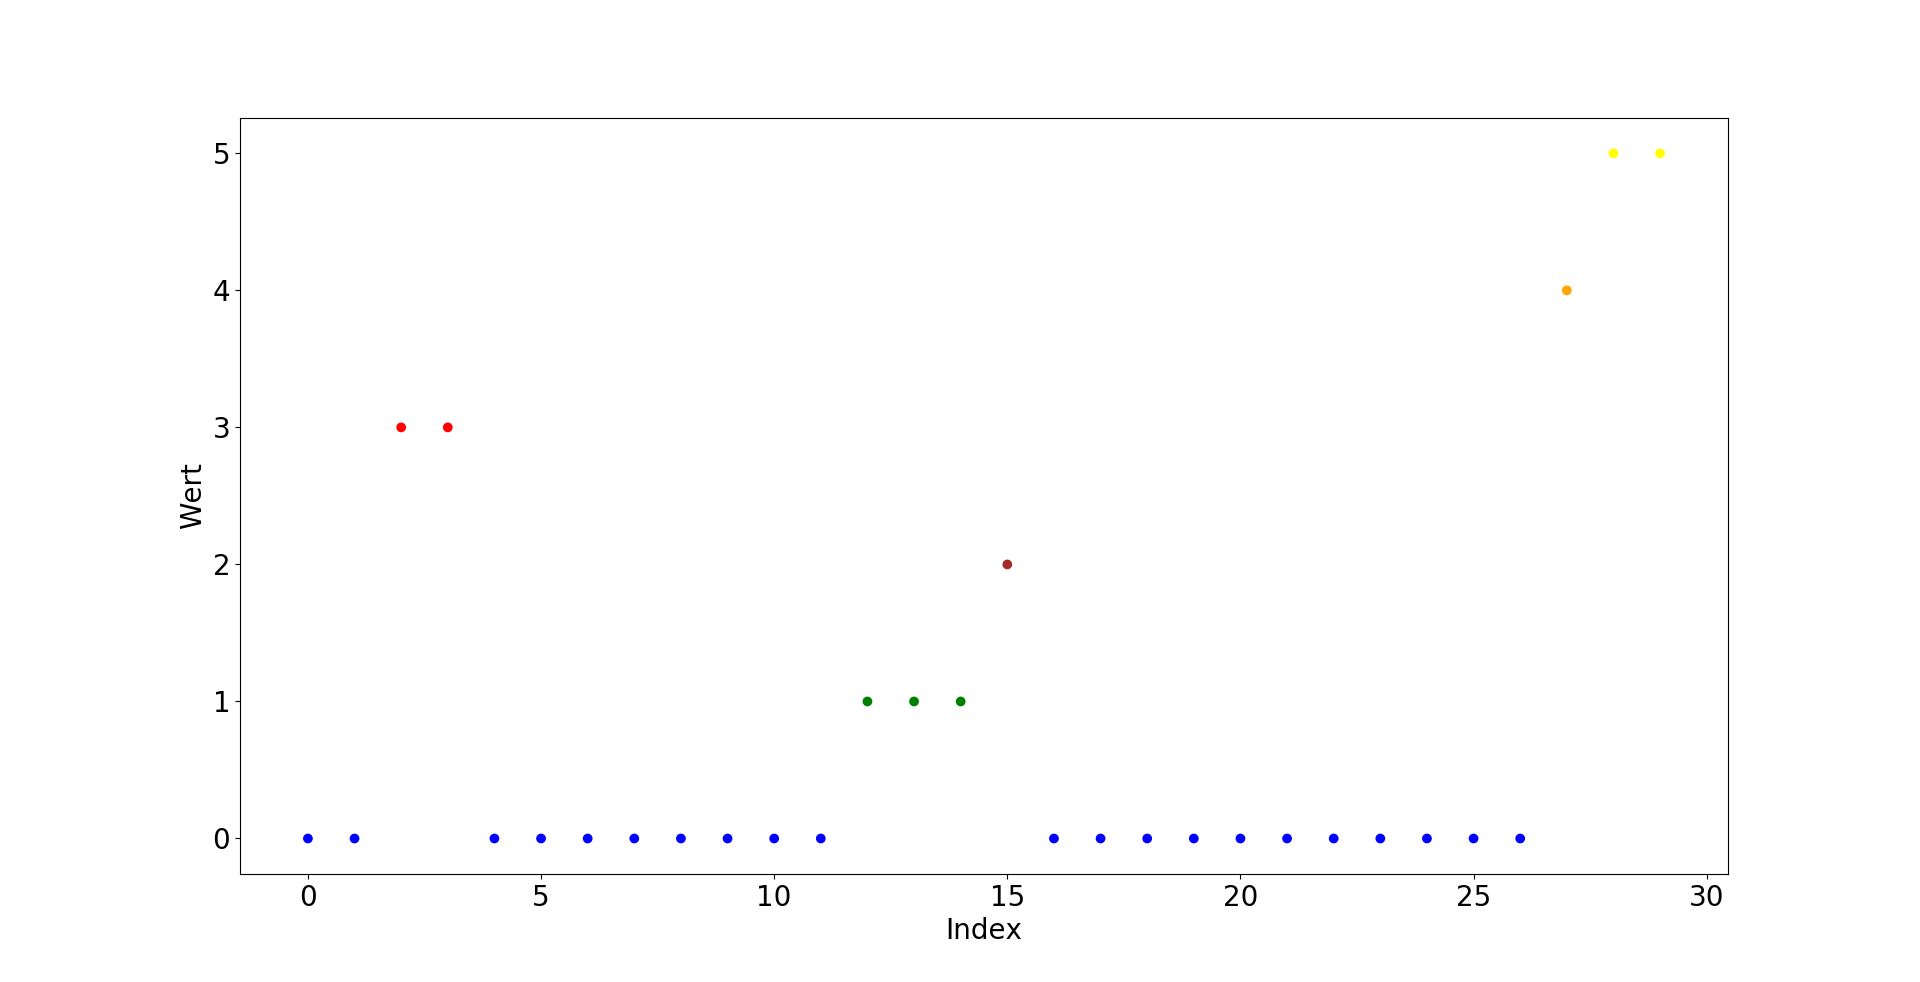
\includegraphics[scale=0.35]{images/Zustandsreduktion/full}
	\caption{Sequenz mit sechs Zuständen}
	\label{fig:full-status}
\end{figure}

\begin{figure}
	\centering
		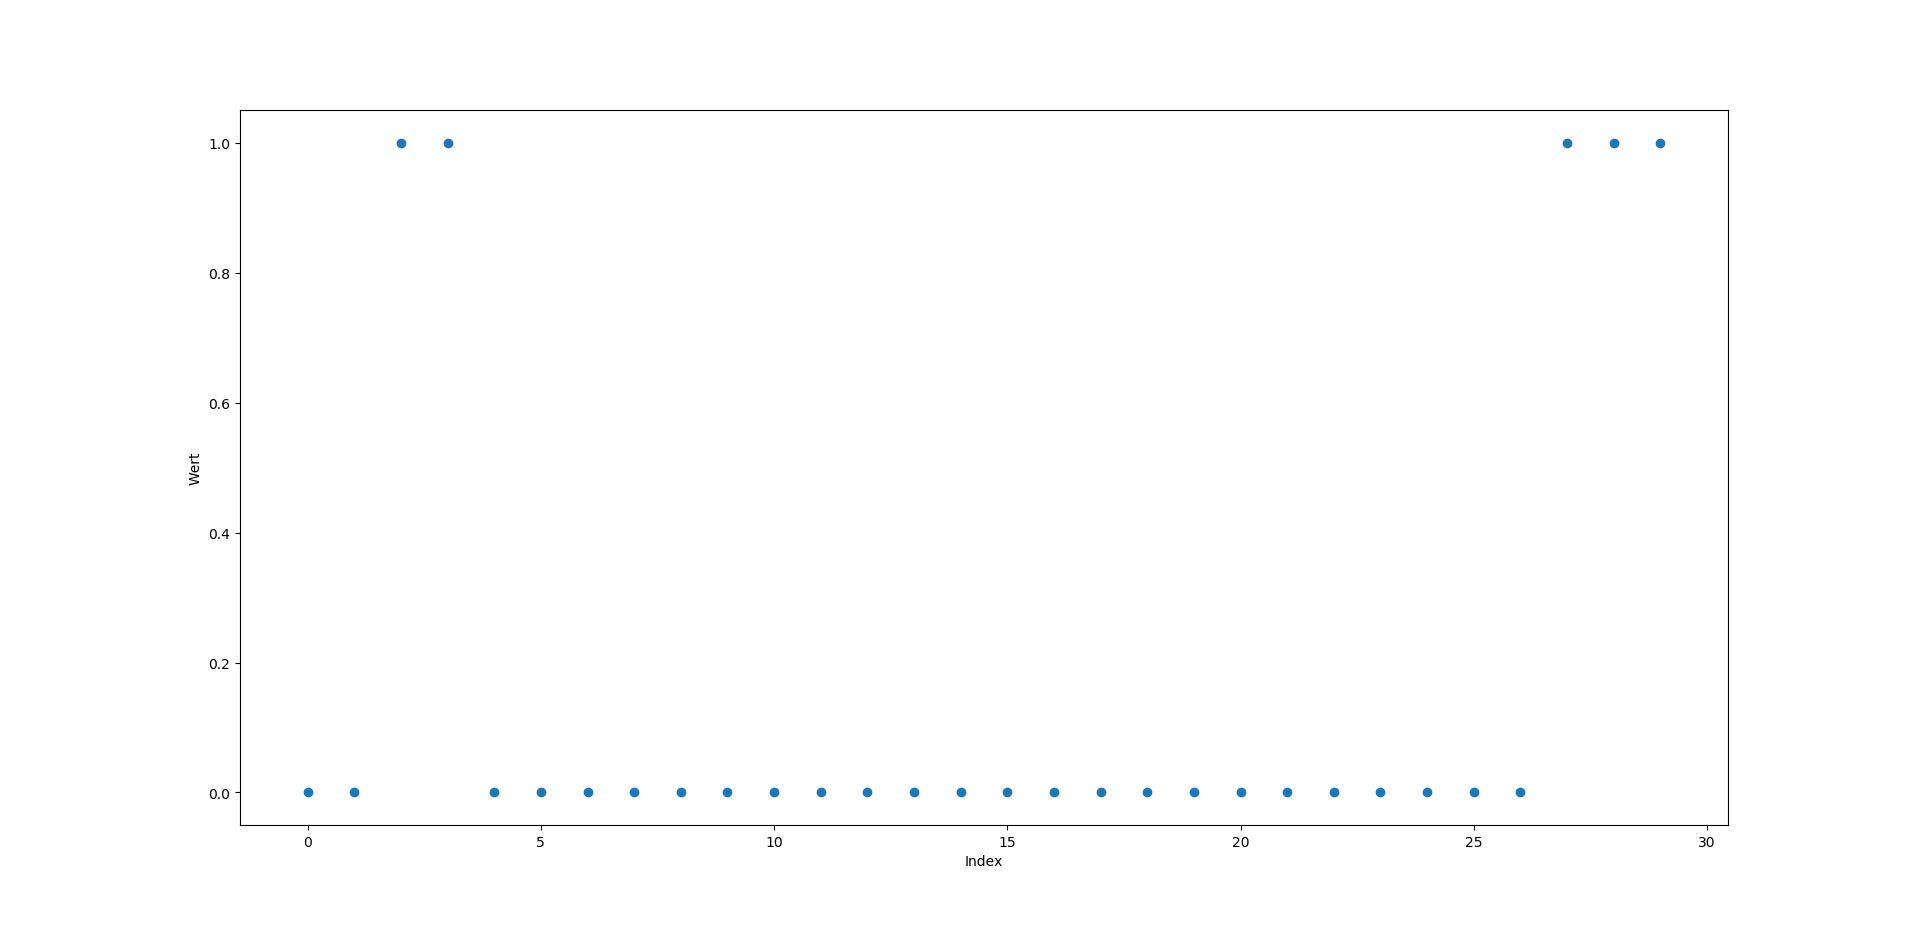
\includegraphics[scale=0.35]{images/Zustandsreduktion/reduced}
	\caption{Sequenz mit zwei Zuständen}
	\label{fig:reduced-status}
\end{figure}

\section{Eigenschaften}
Um Sequenzen oder Teilsequenzen zu klassifizieren, müssen Eigenschaften definiert und voneinander abgegrenzt werden. Dazu werden die \textit{Balance} und \textit{Frequenz} einer Sequenz eingeführt.

Mit der Balance wird das Verhältnis des Vorkommens eines Symbols zur Länge der Sequenz beschrieben. 

\begin{equation}
\label{eq:balance}
Balance(Symbol) = \frac{Anzahl(Symbol)}{Gesamtl\ddot{a}nge\ der\ Sequenz}
\end{equation}

\begin{equation}
\label{eq:binary-balance}
Balance(0) + Balance(1) = 1\ f\ddot{u}r\ \Sigma = [0,1]
\end{equation}

Man kann die Balance somit auch als Maß für die Ausrichtung einer Sequenz zu einem Symbol hin bezeichnen. Die Balance wird nach der Formel \ref{eq:balance} berechnet. Für eine binäre Sequenz gilt zudem Formel \ref{eq:binary-balance}. Mit ihr ist es möglich Balance(1) aus Balance(0) und anders herum zu berechnen.

\begin{theorem}
Aus $s = [1,0,0,0,1,0,1,1,1,1]$ mit $\Sigma = [0,1]$ und der Länge $|s| = 10$ folgen:

$
Balance(0) = \frac{Anzahl(0)}{|s|} = \frac{4}{10} = 0.4
$

$
Balance(1) = \frac{Anzahl(1)}{|s|} = \frac{6}{10} = 0.6
$
\end{theorem}

Daneben ist die Frequenz ist ein Maß für die Aktivität an Wertewechseln innerhalb einer Sequenz. Sie ist das Verhältnis zwischen der Anzahl der Wertewechsel und der Sequenzlänge und wird nach Formel \ref{eq:frequence} berechnet. 

\begin{equation}
\label{eq:frequence}
Frequenz = \frac{Anzahl\ der\ Wertewechsel}{Gesamtl\ddot{a}nge\ der\ Sequenz}
\end{equation}

Ein Wertewechsel tritt auf, wenn ein Element der Sequenz sich von seinem nachfolgendem Element unterscheidet, also $s_{i} \neq s_{i+1}$ ist. In einem Produktionsprozess könnte dies der Zeitpunkt sein, bei dem es zu einer Störung kommt, bzw. eine Störung behoben wurde. Bei einer binären Sequenz handelt es sich um den Wechsel von 0 auf 1, bzw. von 1 auf 0.

\begin{theorem}
Aus $s = [1,0,0,0,0,0,1,1,1,1]$ mit $\Sigma = [0,1]$ und der Länge $|s| = 10$ folgt:

$
Frequenz = \frac{Anzahl\ der\ Wertewechsel}{|s|} = \frac{2}{10} = 0.2
$
\end{theorem}

Somit lassen sich mit Hilfe der Balance und Frequenz Aussagen darüber treffen, wie häufig ein Fehlerzustand in einer Sequenz auftritt und ob es häufig zu Wertewechseln kommt. Dabei bietet es sich an, besonders bei langen Sequenzen, sich auch die Eigenschaften von Teilsequenzen anzuschauen.

\begin{theorem}
Bei $s = [0,0,0,0,0,0,0,0,1,1,1,1,1,1,1,1,1,1,1,1,0,1,0,1,0,1,0,1,0,1]$ mit $\Sigma = [0,1]$ und der Länge $|s| = 30$ werden die fünf Teilsequenzen $t_{0,5}(s)$, $t_{6,11}(s)$, $t_{12,17}(s)$, $t_{18,23}(s)$ und $t_{24,29}(s)$ betrachtet. Mit den Formeln \ref{eq:balance} und \ref{eq:frequence} ergeben sich für jede Teilsequenz sowie die gesamte Sequenz:

\begin{center}
	\begin{tabular}{|c c c|} 
		\hline
		Sequenz & Balance(0) & Frequenz \\
		\hline\hline
		s & $0.4\overline{3}$ & $0.3\overline{6}$ \\ 
		\hline
		$t_{0,5}(s)$ & 1 & 0 \\ 
		\hline
		$t_{6,11}(s)$ & $0.\overline{3}$ & $0.1\overline{6}$ \\
		\hline
		$t_{12,17}(s)$ & 0 & 0 \\
		\hline
		$t_{18,23}(s)$ & $0.\overline{3}$ & $0.\overline{6}$ \\
		\hline
		$t_{24,29}(s)$ & 0.5 & $0.8\overline{3}$ \\
		\hline
	\end{tabular}
\end{center}

Es zeigt sich, dass Balance und Frequenz in den Teilsequenzen teils stark variieren. Damit zeigt sich auch die Wichtigkeit Sequenzen nicht nur als Ganzes, sondern auch deren Verhalten über die Zeit zu betrachten. So sind zu Beginn noch keine Wertewechsel (Frequenz = 0) erkennbar, während zum Ende hin die Sequenz sehr aktiv wird (Frequenz = 0.8$\overline{3}$).
\end{theorem}

\section{Klassifizierung}
Wenn man Sequenzen graphisch darstellt ergeben sich unterschiedliche Muster. Um die Klassifikation von Sequenzen zu erleichtern werden anhand der Balance und Frequenz Klassen für bestimmte Wertebereiche definiert. Die im folgenden vorgenommenen Definitionen haben zur Grundannahme, dass es sich um binäre Sequenzen handelt.

Der kleinste Wert für die Balance oder Frequenz ist 0 und der größte kleiner gleich 1. Eine Sequenz mit einer niedrigen, bzw. hohen Balance wird als unausgeglichen beschrieben, während ein Wert um die 0.5 als ausgeglichen gilt. Dieser Ausgleich bezieht sich letztlich auf die Verteilung der Nullen und Einsen. Eine detaillierte Auflistung der unterschiedlichen Wertebereiche findet sich in Tabelle \ref{tab:balance}. 

\begin{table}
\label{tab:balance}
	\begin{center}
		\begin{tabular}{|c c|} 
			\hline
			Balance & Beschreibung \\
			\hline\hline
			$0 \leq B < 0.4$ & unausgeglichen \\ 
			\hline
			$0.4 \leq B \leq 0.6$ & ausgeglichen \\
			\hline
			$0.6 < B \leq 1$ & unausgeglichen \\
			\hline
		\end{tabular}
		\caption{Balance}
	\end{center}
\end{table}

Da mit der Frequenz ein Maß für die Wertewechsel innerhalb einer Sequenz bildet, entspricht ein Wert gegen 0 einer sehr inaktiven Sequenz mit nur sehr wenigen bis keinen Wertewechseln. Ein Wert von 1 steht hingegen für eine hochfrequente Sequenz, in der sehr viel Wertewechsel stattfinden. Eine detaillierte Auflistung der unterschiedlichen Wertebereiche findet sich in Tabelle \ref{tab:frequence}. 

\begin{table}
\label{tab:frequence}
	\begin{center}
		\begin{tabular}{|c c|} 
			\hline
			Frequenz & Beschreibung \\
			\hline\hline
			$0 \leq F \leq 0.25$ & niederfrequent \\ 
			\hline
			$0.25 < F < 0.75$ & mittelfrequent \\
			\hline
			$0.75 \leq F < 1$ & hochfrequent \\
			\hline
		\end{tabular}
		\caption{Frequenz}
	\end{center}
\end{table}

Nachdem die unterschiedlichen Wertebereiche der Eigenschaften beschrieben wurden, können nun markante Grundmuster mit ihrer Hilfe klassifiziert werden.

Eine Sequenz befindet sich fast ausschließlich in einem Zustand. Änderungen treten fast gar nicht und wenn doch nur kurz auf. Dieses Muster wird \textit{Ausreißer} genannt und ist in Abbildung \ref{fig:ausreisser} dargestellt. Bei maschinellen Prozessen könnte man dieses Muster bei einer Maschine, welche im Regelbetrieb arbeitet und kurz einen Fehler wirft, beobachten. Wichtig dabei ist, dass schnell wieder ein Sprung in den Ausgangszustand stattfindet. Die Balance einer solchen Sequenz ist unausgeglichen und die Frequenz sehr niedrig.\\

Ein weiteres Grundmuster ist in Abbildung \ref{fig:zittern} dargestellt. Dieses zeigt einen regelmäßigen Wechsel zwischen den zwei möglichen Zuständen und wird als \textit{Zittern} bezeichnet. Dieses Verhalten ist eher untypisch für Produktionsmaschinen und dürfte nicht oft beobachtet werden. Hier wäre ein Rückschluss auf eine defekte Sensorik naheliegend. Solche Sequenzen haben eine Balance von ca. 0.5 sowie eine hohe Frequenz .\\ 

Bei dem dritten Muster befindet sich eine Sequenz zuerst in einem Zustand und verharrt nach einem Wertewechsel im anderen. Abbildung \ref{fig:wechsel} zeigt dieses Muster. In der Praxis kann so ein Muster auftreten, wenn eine Maschine im Regelbetrieb arbeitet und auf Grundlage eines Fehlers längere Zeit ausfällt. Durch diesen \textit{Wechsel} ergibt sich zudem der Name dieses Musters.

\begin{figure}
	\centering
		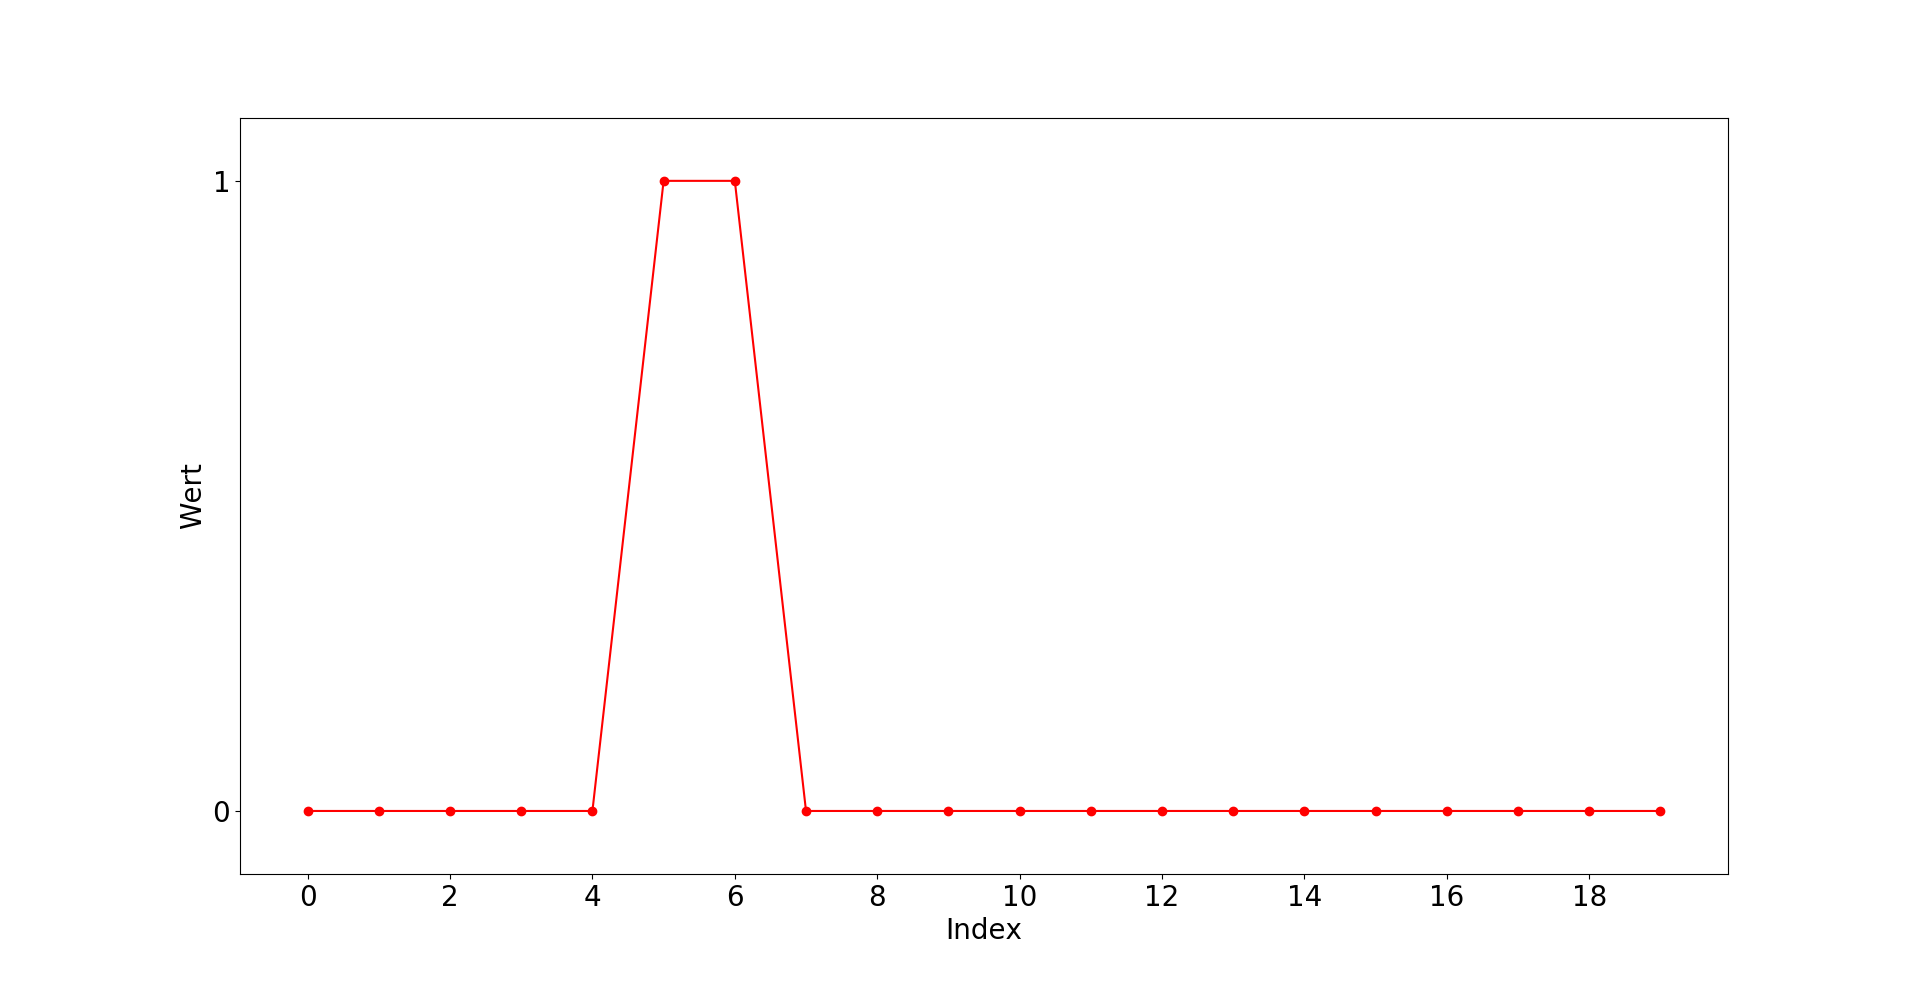
\includegraphics[scale=0.5]{images/Klassifizierung/ausreisser}
	\caption{Sequenz mit einem Ausreißer}
	\label{fig:ausreisser}
\end{figure}

\begin{figure}
	\centering
		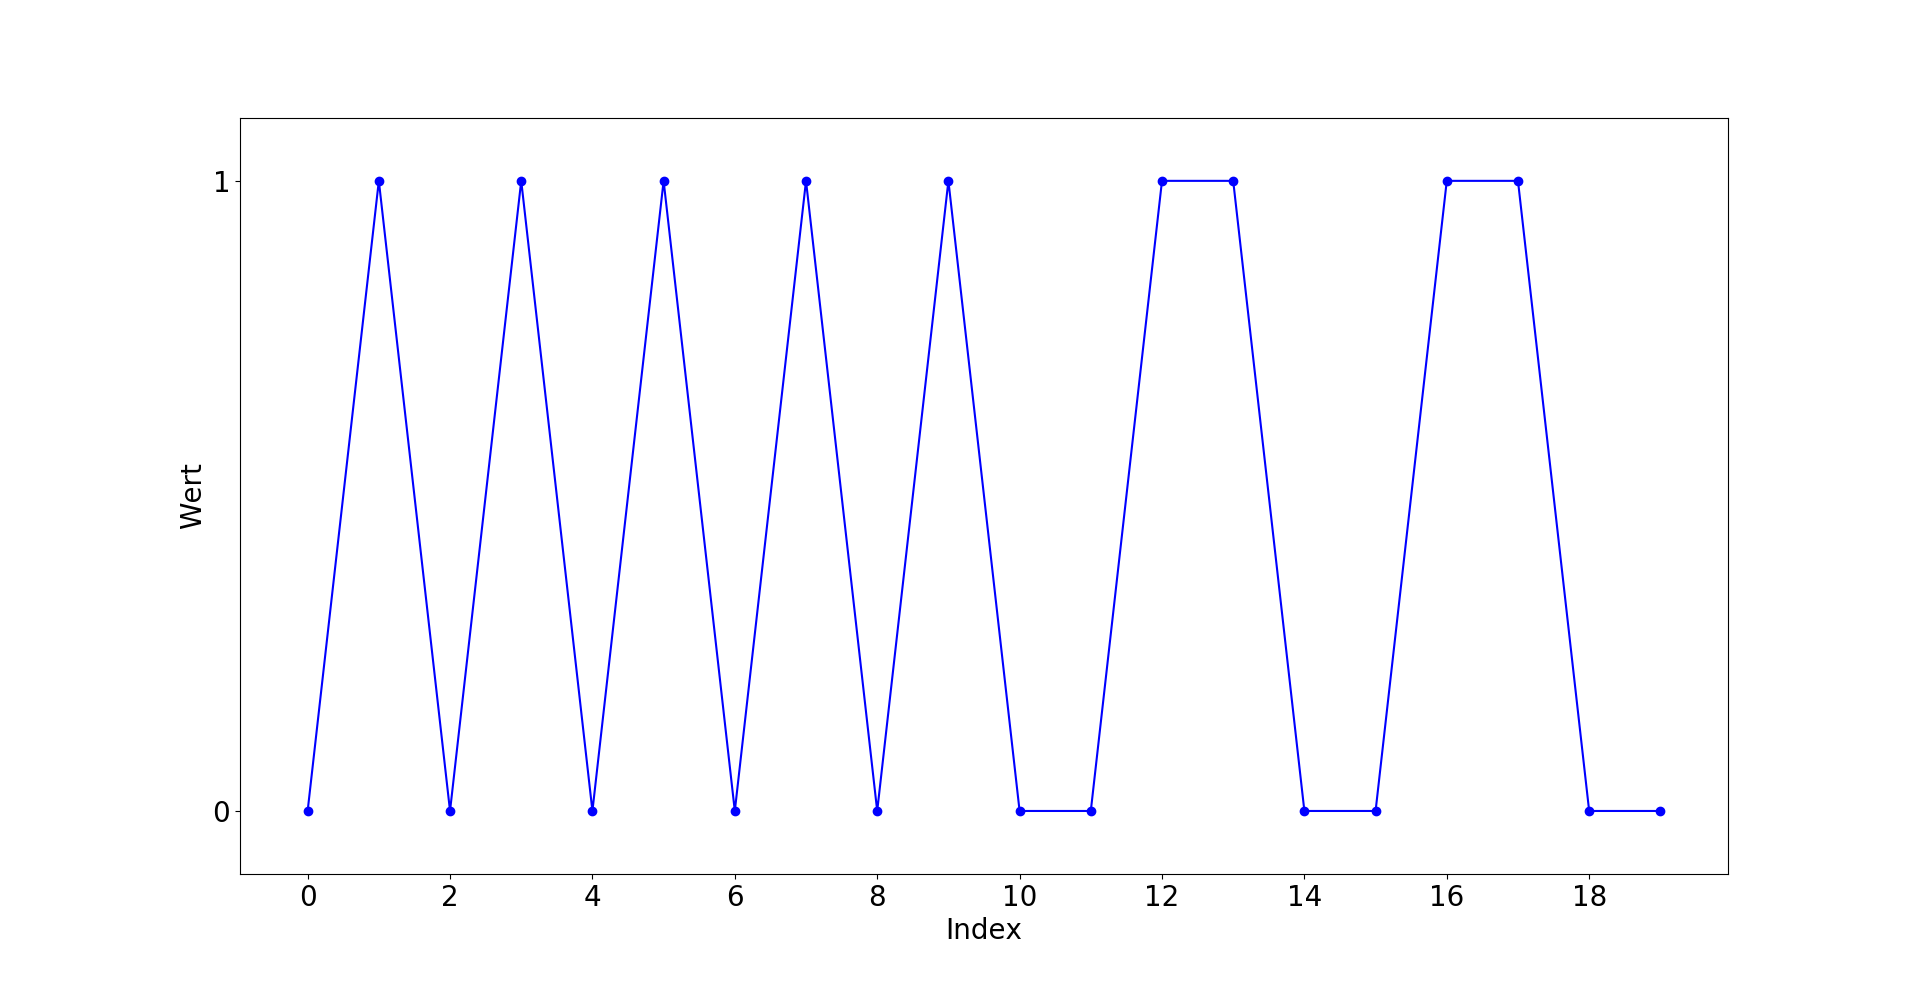
\includegraphics[scale=0.5]{images/Klassifizierung/zittern}
	\caption{Sequenz mit einem Zittern}
	\label{fig:zittern}
\end{figure}

\begin{figure}
	\centering
		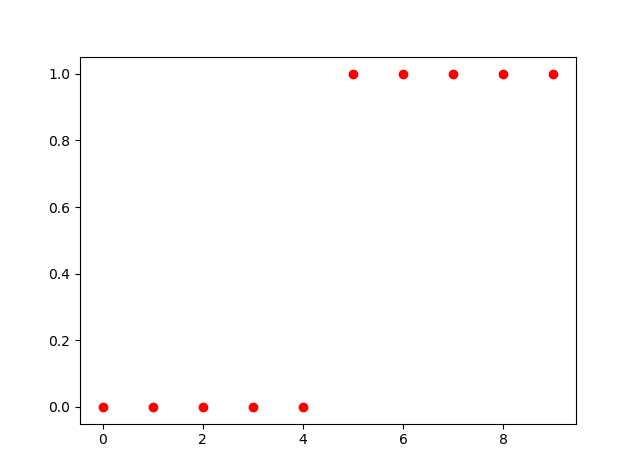
\includegraphics[scale=0.5]{images/Klassifizierung/wechsel}
	\caption{Sequenz mit einem Wechsel}
	\label{fig:wechsel}
\end{figure}